\mysection{Travel}{movement-travel}

\ed{This mechanic is taken from John Carr's \href{https://ageofruins.wordpress.com/2012/10/18/deck-of-many-threats-wilderness-encounters-based-on-playing-cards-plus-a-simple-system-for-provisions/}{Age of Ruins}}

Journeys consist of a number of routes (called Legs) to get from one point to another.  These routes are sometimes defined ("the Iron Road", "the High Pass", etc.) but can make routes of your own by looking at a map.  For example, "we must bear north, following the Miskatonic River, until we reach the mouth of the bay.  From there we will follow the coast west until we reach the point where the Iron Road meets Portsmouth, then follow the road south to Erl" is a journey of 3 legs (north to the bay, west to the road, south to Erl).  At the end of each Leg, you must roll your Party Provisions \UD - just before you do, if someone can \RO using their Skill: Travel, the provisions only move \DCDOWN on a roll of a 1 (instead of a 1 or 2).

To figure out what happens on a Journey, you'll need a deck of cards.  Leave the Jokers in.

\mysubsection{Legs}{movement-travel-legs}

Roughly speaking, each leg of a journey is about 5-10 Days (50-100 leagues) (this can change at the Arbiter's discretion).  The Arbiter should assign a Danger value to each leg on a scale of 1 (the Gold Road) to 6 (trog-infested swamps).  The Arbiter can tell you the Danger value of each Leg at her discretion. 


At the start of each Leg, draw a number of cards equal to the Leg's \mybold{Danger}. You use the same deck of cards for the entire Journey, so don't shuffle cards back in until the Journey's complete. 

\cbreak

The Arbiter will flip each card one at a time. If an Ace, Joker, or face card is flipped you must first check the suit:

  \mytable{Y Y}{
    \thead{Suit} & \thead{Effect} \\
  }{
    \mybold{Clubs} & Lose Provisions \\
    \mybold{Diamonds} & Bad weather  \\
    \mybold{Hearts} & You get lost or are off course \\
    \mybold{Spades} & You run into some hostiles  \\
    \mybold{Jokers} & You stumble on something interesting ... \\
  }

  followed by the type of card it is to indicate when the event takes place:


  \mytable{Y Y}{
    \thead{Face} & \thead{Effect} \\
  }{
    \mybold{Jack} & Predawn \\
    \mybold{Queen} & Morning  \\
    \mybold{King} & Afternoon \\
    \mybold{Ace} & Evening  \\
    \mybold{Joker} & Arbiter's Choice \\
  }     


  \mysubsection{Lose Provisions}{movement-travel-provisions}

  Rats ate the flour; the mule stumbled and dropped the bacon in a river; someone ate more than their fair share along the way.  Move your Party Provisions \DCDOWN.  Someone in the Band can try a \RO using their \mylink{Skill: Travel}{adventurer-skills} to prevent this from happening.

  \mysubsection{Bad Weather}{movement-travel-weather}

  You hit appropriate bad weather (snowstorm, sandstorm, torrential downpour, etc).  Someone in the Band must try their Skill: Travel.  If they succeed, nothing happens.  If they fail, roll a d3:  1) you lose provisions (see above) 2) you're lost (see below); 3) you run into hostiles (see below)


\begin{figure*}
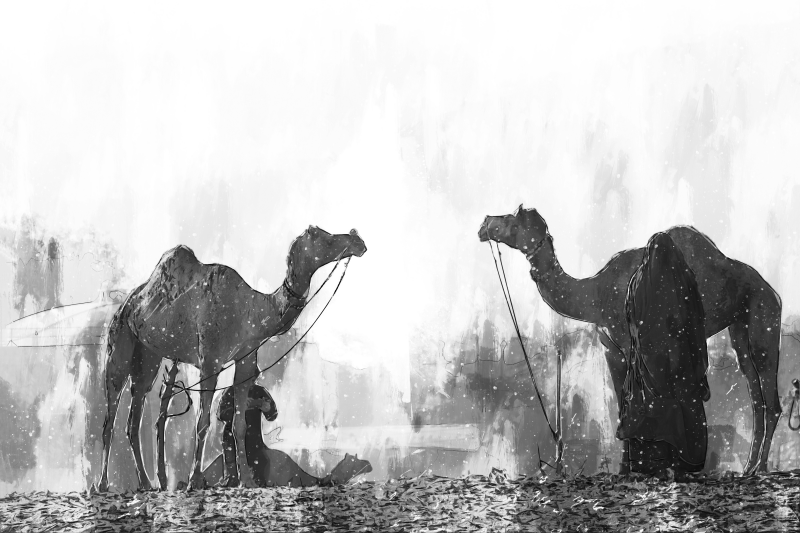
\includegraphics[width=\textwidth]{movement/TravelCamels}
\end{figure*}

\newpage 

  \mysubsection{Lost}{movement-travel-lost}

  This can only happen if you are \myital{not} on a road. If you're traveling by road, you can ignore this result.

  Someone in the Band must try their Skill: Travel.  If they succeed, you get back on track.  If they fail, the Arbiter will move you in a random direction (on a hex map, roll a d6 and move the party in that direction) and will draw another card and put it on the bottom of the pile. Continue in this way until someone succeeds at their Skill: Travel try to figure out where they are.


  \mysubsection{Hostiles}{movement-travel-hostiles}

  The Arbiter will roll on the random monster table for this area (or make something up).

\cbreak

  \mysubsection{Something Interesting}{movement-travel-pointofinterest}

  This can only happen if you are \myital{not} on a road. If you're traveling by road, ignore this result.  This is entirely up to the Arbiter, but might include: an entrance to a small dungeon, a weird shrine to a lost god, an "abandoned" gnoll war camp, etc.


  \mysubsection{We're Out of Food}{movement-travel-starvation}

  If you run out of food, time switches to Game Time.  The Arbiter should determine how many Days the party is from their destination (the party can cover 10 leagues / 1 hex on a road every Day, whereas it might take 3 Days to cover 1 hex in the mountains).  The party should now follow the rules as if they were in a wilderness dungeon, including rolling Personal Provisions, using their Skill: Bushcraft, etc. 

